\documentclass{article}

% if you need to pass options to natbib, use, e.g.:
% \PassOptionsToPackage{numbers, compress}{natbib}
% before loading nips_2016
%
% to avoid loading the natbib package, add option nonatbib:
% \usepackage[nonatbib]{nips_2016}

% \usepackage{nips_2016}

% to compile a camera-ready version, add the [final] option, e.g.:
\usepackage[final]{nips_2016}

\usepackage[utf8]{inputenc} % allow utf-8 input
\usepackage[T1]{fontenc}    % use 8-bit T1 fonts
\usepackage{hyperref}       % hyperlinks
\usepackage{url}            % simple URL typesetting
\usepackage{booktabs}       % professional-quality tables
\usepackage{amsfonts}       % blackboard math symbols
\usepackage{nicefrac}       % compact symbols for 1/2, etc.
\usepackage{microtype}      % microtypography
\usepackage{graphicx}
\usepackage{caption}
\usepackage{subcaption}

\title{Texture sequence generation using convolutional networks}

% The \author macro works with any number of authors. There are two
% commands used to separate the names and addresses of multiple
% authors: \And and \AND.
%
% Using \And between authors leaves it to LaTeX to determine where to
% break the lines. Using \AND forces a line break at that point. So,
% if LaTeX puts 3 of 4 authors names on the first line, and the last
% on the second line, try using \AND instead of \And before the third
% author name.

\author{
  Thomas George\thanks{Use footnote for providing further
    information about author (webpage, alternative
    address)---\emph{not} for acknowledging funding agencies.} \\
  Université de Montréal\\
  \texttt{tfjgeorge@gmail.com} \\
  %% examples of more authors
  %% \And
  %% Coauthor \\
  %% Affiliation \\
  %% Address \\
  %% \texttt{email} \\
  %% \AND
  %% Coauthor \\
  %% Affiliation \\
  %% Address \\
  %% \texttt{email} \\
  %% \And
  %% Coauthor \\
  %% Affiliation \\
  %% Address \\
  %% \texttt{email} \\
  %% \And
  %% Coauthor \\
  %% Affiliation \\
  %% Address \\
  %% \texttt{email} \\
}

\begin{document}
% \nipsfinalcopy is no longer used

\maketitle

\begin{abstract}
  TODO
  
  An emphasize is put on understanding the different issues that arise when implementing and training texture generator networks.
\end{abstract}

\section{Introduction}

TODO

\section{Feed-forward texture synthesis}

\subsection{Using convolutional networks as feature descriptors}

Following the success of convolutional neural networks for solving image classification tasks, a lot of pretrained networks for different architectures have been made publicly available. This convolutional networks are powerful feature extractors that start from a raw pixel image and sequentially build new representations at each layer that are then used by a standard logistic regression as a top layer to predict a class from a given set.

While the representations in the first layers are low level representations that describe the edges orientation and the colors of the images, deeper representations represent more abstract objects such as complex shapes and arrangements of colors. Thus a texture synthesis task can be thought as finding an image with a similar texture to a base image, the similarity being measured using the metrics based on this representations using the metrics described in the following paragraphs.

\subsection{Formulating texture generation as an optimization problem}

TODO

In the following we will refer to the network used to define the lost function as the descriptor network.

\subsection{Choosing layer to best describe a texture}

A problem arising with this technique is that we have to choose which layer best describe a texture.

Proposed solution : for each layer compute distance between gram matrix for layer for image and flipped image

The network we use to extract our descriptors was pre trained on ImageNet. 

\subsection{Texture synthesis strategies}

Gatys et al. proposed a strategy that consists in starting from a random image and iterate gradient descent steps on the value of the pixels to find a minimum of the loss function. This gives results that are visually appealing and is quite simple to train using a framework where getting the gradients by back-propagation is easy to do such as Theano. A caveat with this procedure is that it takes a full learning run each time you want to generate a new texture.

A follow-up was proposed by Ulyanov et al., who describe a generator network that uses random noise images as input to directly output a texture image. The texture generation only needs a feed forward pass which allows to generate images in near real time. This network is described in the following section.



\section{Generator network}

\subsection{Architecture}

\subsection{Choosing the number of filters for each resolution}

Choosing the number of filters used at each resolution is also a difficult problem with no real answer. As a heuristic, we consider the following: in our descriptor network, we made a choice for which layers to choose to best describe a texture. The choice of filters must be done with the idea that at each layer chosen in the descriptor network corresponds a spatial resolution, i.e. each time we do subsampling the spatial resolution is divided by 2. We should add more filters for the corresponding resolution in the generator network.

\subsection{Training}

\subsection{Issues}
\subsubsection{Overfitting}

A global minimum to this optimization problem is obvious : take the original texture image and you get a zero loss function. This is not desired, as we want the generator to be able to generate new texture images, not to reproduce an existing image. The optimization procedure does not seem to find this kind of minimum however.

But an issue that arises is that the biases in the convolution layers learn a local optimum. This usually happens along the edges of the image and we hypothesize this is an effect of the border convolutions being zero-padded (\label{fig:overfit}). A solution could be to add a regularization term that penalizes images to be too close in a mini batch but this has not being explored due to lack of time. Another simpler solution could be to regularize the norm of the biases.

To counter this issue we simply did not use bias, even if it allowed for faster initial convergence.

\begin{figure}[h]
    \centering
    \begin{subfigure}[b]{0.48\textwidth}
        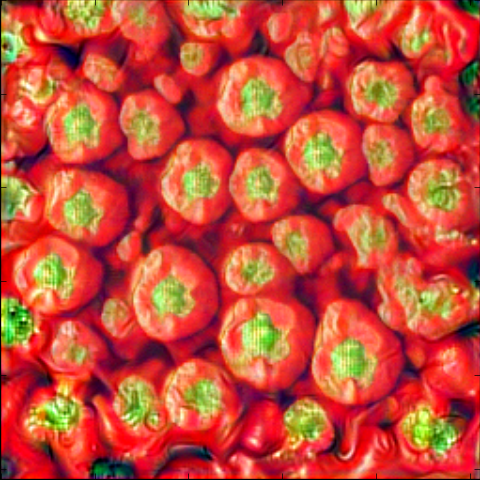
\includegraphics[width=\textwidth]{overfit1}
    \end{subfigure}
    \begin{subfigure}[b]{0.48\textwidth}
        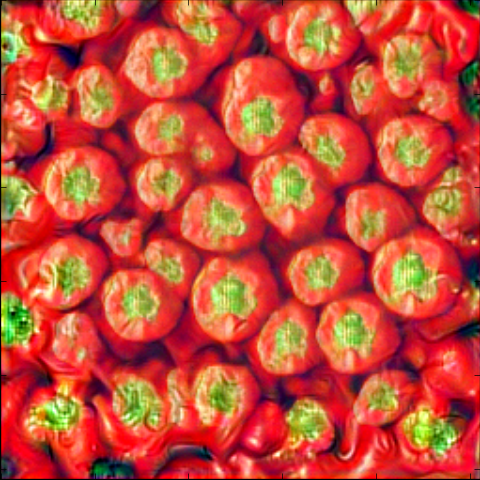
\includegraphics[width=\textwidth]{overfit2}
    \end{subfigure}
   
    \caption{Two images generated using two different noise images using a trained network that has learned a good minimum for the biases. Notice how both images are similar around the edges and especially in the corners, while being really different in the middle.}\label{fig:overfit}
\end{figure}

\subsubsection{Capacity}

number of 

\subsubsection{Memory}

\section{Video textures}

\subsection{Motivation}
Once we have a base texture generator, we can think of it as a way to sample from a texture manifold lying in the space of pixels. The random noise images given as input of the generators can be considered as latent variables that determine where to pick the sample along that manifold. By interpolating linearly between the pixels values for two random images we can get a sequence of images with each consecutive image being very similar to the previous one, and in the meantime being in the manifold of images that have a similar texture to the target texture. This idea motivates building sequences of frames that transform a texture image into a new texture image.

We did not intend to generate realistic videos. As a simple example, think of the transformation between two textures representing red peppers. We do not see red pepper turn into air then back to red pepper in the real world. However we find the results visually appealing. Note that for some example (e.g. water) the video could look somehow realistic.

\subsection{Procedure}

This section describes the procedure used to generate sequences of transformations between two texture images. We first sample two sets of random images of required sizes (256, 128, 64, 32, 16). We then interpolate between these two images, so that the random images given as input to the generator network are given by:
$$x^{(i)}(t) = t \, x^{(i)}_1 + (1-t) \,  x^{(i)}_2 \, , t \in [0,1]$$

We then construct a sequence with the output images. The frame rate is 30 per second and we increase $t$ by $0.01$ at each time step.

\subsection{Experiments}

\section*{References}

References follow the acknowledgments. Use unnumbered first-level
heading for the references. Any choice of citation style is acceptable
as long as you are consistent. It is permissible to reduce the font
size to \verb+small+ (9 point) when listing the references. {\bf
  Remember that you can use a ninth page as long as it contains
  \emph{only} cited references.}
\medskip

\small

[1] Alexander, J.A.\ \& Mozer, M.C.\ (1995) Template-based algorithms
for connectionist rule extraction. In G.\ Tesauro, D.S.\ Touretzky and
T.K.\ Leen (eds.), {\it Advances in Neural Information Processing
  Systems 7}, pp.\ 609--616. Cambridge, MA: MIT Press.

[2] Bower, J.M.\ \& Beeman, D.\ (1995) {\it The Book of GENESIS:
  Exploring Realistic Neural Models with the GEneral NEural SImulation
  System.}  New York: TELOS/Springer--Verlag.

[3] Hasselmo, M.E., Schnell, E.\ \& Barkai, E.\ (1995) Dynamics of
learning and recall at excitatory recurrent synapses and cholinergic
modulation in rat hippocampal region CA3. {\it Journal of
  Neuroscience} {\bf 15}(7):5249-5262.

\end{document}
